\documentclass[10pt,xcolor={svgnames}]{beamer}
%\usefonttheme[onlymath]{serif}
%%%%% Colors
\usetheme{Dresden}%\usetheme{Madrid}
\colorlet{beamer@blendedblue}{green!55!black}
%%%%%

%%%%% Other 
\beamertemplatenavigationsymbolsempty
\addtobeamertemplate{navigation symbols}{}{%
    \usebeamerfont{footline}%
    \usebeamercolor[fg]{footline}%
    \hspace{1em}%
    \insertframenumber/\inserttotalframenumber
}
\usepackage{hyperref, url}
%\usepackage[symbol]{footmisc}

\definecolor{pine_green}{HTML}{007935}
\hypersetup{colorlinks,breaklinks,linkcolor=white,urlcolor=orange,citecolor=black}
\renewcommand\thefootnote{\textcolor{pine_green}{\arabic{footnote}}}
\setbeamercolor{alerted text}{fg=pine_green}

\renewcommand{\i}{\mathnormal{I}}

\usepackage{cancel}
\usepackage{ulem}
\usepackage{multirow}
\usepackage{mathtools}
\usepackage{makecell}
\DeclarePairedDelimiter{\abs}{\lvert}{\rvert}
\renewcommand{\epsilon}{\varepsilon}
\setbeamertemplate{itemize subitem}{\textbullet}
\setbeamertemplate{itemize subsubitem}{$\circ$}

%https://tex.stackexchange.com/questions/289542/auto-resizing-parenthesis-in-math-formulas
% \usepackage{amsmath} for testing
\newcommand*\autoop{\left(}
\newcommand*\autocp{\right)}
\newcommand*\autoob{\left[}
\newcommand*\autocb{\right]}
\AtBeginDocument {%
   \mathcode`( 32768
   \mathcode`) 32768
   \mathcode`[ 32768
   \mathcode`] 32768
   \begingroup
       \lccode`\~`(
       \lowercase{%
   \endgroup
       \let~\autoop
   }\begingroup
       \lccode`\~`)
       \lowercase{%
   \endgroup
       \let~\autocp
   }\begingroup
       \lccode`\~`[
       \lowercase{%
   \endgroup
       \let~\autoob
   }\begingroup
       \lccode`\~`]
       \lowercase{%
   \endgroup
       \let~\autocb
   }}

\delimiterfactor 1001

\makeatletter
% for amsmath "compatibility" (not sophisticated)
% \usepackage{amsmath}
\AtBeginDocument {%
          \def\resetMathstrut@{%
           \setbox\z@\hbox{\the\textfont\symoperators\char40}%
           \ht\Mathstrutbox@\ht\z@ \dp\Mathstrutbox@\dp\z@}%
}%
\makeatother
%%%%%

%%%%% Greying out/invisible Slides
%\setbeamercovered{invisible}
%\setbeamercovered{%
%  again covered={\opaqueness<1->{15}}}
  
%%%%%







%%%%% Footnotes and captions
%\usepackage[utf8]{inputenc}
\usepackage{caption}
\usepackage{comment}
\setbeamerfont{footnote}{size=\tiny}
\setbeamerfont{caption}{size=\small}
%\setbeamerfont{normal text}{size=\small}
\setbeamerfont{itemize/enumerate body}{size=\small}
\setbeamerfont{itemize/enumerate subbody}{size=\footnotesize}
%%%%%


%%%%
\usepackage{booktabs}
\usepackage{multirow,bigstrut}
\usepackage{tabu}

%%%%



%Information to be included in the title page:
\title[Connor Wiegand]{Intro to Economic Analysis: Microeconomics}
\subtitle{EC 201 - Day 11 Slides}
\author[EC 201]{Connor Wiegand}
\institute[]{Department of Economics - University of Oregon}
\date{1 November 2021}


\begin{document}

\frame{\titlepage}

\section*{Recall}

\begin{frame}{Logistics}
    \begin{itemize}
        \item Official homework 4 due this Saturday at 11:59pm, covering last week's material
        \item Next news assignments posted, due today
        \item Midterm is a week from today -- Wednesday, November 3rd 
        \begin{itemize}
            \item Bring non-graphing, non-algebra calculator
            \item Bring \#2 Pencil (yes it has to be \#2)
            \item Bring ID
            \item All of these items are required; I will try to bring spares, but I cannot promise anything
        \end{itemize}
    \end{itemize}
\end{frame}

\section*{A Real World Example}

\begin{frame}{``The Labor Shortage"}
    \begin{itemize}[<+->]
        \item Frequently in the news lately, you might have heard about the supposed ``labor shortage"
        \item Recall: If a price control is effective, which causes a shortage/surplus?
        \begin{itemize}
            \item Effective floors cause surpluses
            \item Effective ceilings cause shortages
        \end{itemize}
        \item If a price control is ineffective, which causes a shortage/surplus?
        \begin{itemize}
            \item Neither: ineffective price controls do not impact the market
        \end{itemize}
        \item Which do we have: a price floor or a price ceiling?
        \begin{itemize}
            \item The minimum wage is a price \underline{floor}, on the price of labor
        \end{itemize}
        \item Is it effective?
    \end{itemize}
\end{frame}

\begin{frame}{The Labor Market}
    \begin{itemize}[<+->]
        \item Let's start by graphing a hypothetical labor market, with the price of labor (a wage) on the $y$-axis, and the quantity of labor on the $x$-axis
        \begin{figure}
            \centering
            \includegraphics[width=7cm]{lab unreg.pdf}
        \end{figure}
        \item Different from usual graphs: suppliers are the workers, the individuals in the market, while demanders are firms, the businesses in the market
    \end{itemize}
\end{frame}


\begin{frame}{Case 1: A Binding Minimum Wage}
    \begin{itemize}[<+->]
        \item Let's start by assuming that the minimum wage (price floor) is effective
        \item We can use our previous graph, and let's say we have a \$12/hr minimum wage:
        \begin{figure}
            \centering
            \includegraphics[width=8cm]{Lab binding.pdf}
        \end{figure}
    \end{itemize}
\end{frame}

\begin{frame}{Case 1 (cont.)}
\begin{figure}
    \centering
    \includegraphics[width=7cm]{Lab binding.pdf}
\end{figure}
    \begin{itemize}[<+->]
        \item What does quantity supplied appear to be? 
        \begin{itemize}
            \item 300. Remember, this is how much total work laborers are supplying, at a price of $\$12/hr$
        \end{itemize}
        \item What does quantity demanded appear to be? 
        \begin{itemize}
            \item 175. Remember, this is how much total work firms are demanding, at a price of $\$12$/hr
        \end{itemize}
    \end{itemize}
\end{frame}

\begin{frame}{Case 1 (conclusion)}
\begin{figure}
    \centering
    \includegraphics[width=7cm]{Lab binding.pdf}
\end{figure}
    \begin{itemize}[<+->]
        \item Based on this figure and your answers to the previous questions, is there a surplus or a shortage?
        \item What is a surplus in labor called?
        \begin{itemize}
            \item Unemployment
            \item In reality, it is up for debate in the data whether or not an effective minimum wage leads to an increase in unemployment (the same is true for increasing prices)
        \end{itemize}
        \item In any case, an effective minimum wage should not lead to a labor shortage
    \end{itemize}
\end{frame}

\begin{frame}{Case 2 -- A Non-Binding Minimum Wage}
    \begin{itemize}[<+->]
        \item Let's suppose instead that the price floor on wages was \underline{ineffective}, i.e. below market equilibrium
        \item Let's use the same price floor, \$12, but with different supposed data to generate supply and demand
        \item Here is the unregulated market:
        \begin{figure}
            \centering
            \includegraphics[width=7cm]{Lab 2 unreg.pdf}
        \end{figure}
    \end{itemize}
\end{frame}

\begin{frame}{Case 2 (cont.)}
    \begin{itemize}[<+->]
        \item What are $Q_{S}$ and $Q_{D}$?
        \begin{itemize}
            \item $Q_{S}=160$ and $Q_{D}=220$?
            \item NO! We are in equilibrium, because the price floor is non-binding!
        \end{itemize}
        \visible<4->{
        \begin{figure}
            \centering
            \includegraphics[width=7cm]{lab 2 ineff.pdf}
        \end{figure}
        $Q_{S}=Q_{D}=200$}
    \end{itemize}
\end{frame}

\begin{frame}{Case 2 (conclusion)}
\begin{figure}
    \centering
    \includegraphics[width=7cm]{Lab binding.pdf}
\end{figure}
    \begin{itemize}[<+->]
        \item Based on this figure and your answers to the previous questions, is there a surplus or a shortage?
        \begin{itemize}
            \item A: Neither
        \end{itemize}
        \item Thus, regardless of whether or not the minimum wage is binding, we shouldn't see a shortage in labor coming from a minimum wage
    \end{itemize}
\end{frame}

\begin{frame}{Labor Market with Shortage}
    \begin{itemize}[<+->]
        \item And let's just say there is a shortage anyway, we just don't know why
        \item I'll use the previous hypothetical market, and numbers we already have
        \item Reminder: when do we have a shortage?
        \begin{itemize}
            \item When the price is below equilibrium
        \end{itemize}
        \begin{figure}
            \centering
            \includegraphics[width=6cm]{lab 2 shortage.pdf}
        \end{figure}
        \item What should we do?
    \end{itemize}
\end{frame}

\begin{frame}{Labor Market with Shortage}
    \begin{itemize}[<+->]
        \item Recall: under a shortage, whose ``responsibility" is it to get us back to equilibrium?
        \item The demand side of the market (consumers) are responsible for increasing their price offers in order to get the market back to equilibrium
        \begin{itemize}
            \item Recall: Producers are always glad to take higher prices. Hence, it is the consumers job in this case to offer them. In a surplus, it is the producers job to make lower offers
        \end{itemize}
        \begin{figure}
            \centering
            \includegraphics[width=6cm]{lab 2 shortage arrow.pdf}
        \end{figure}
        \item What does that mean in this case?
    \end{itemize}
\end{frame}

\begin{frame}{Labor Market with Exogenous Shortage}
    \begin{itemize}[<+->]
        \item What does that mean in this case?
        \begin{itemize}
            \item Even if we had a labor shortage, the consumers (\textit{firms}, in this case) should be offering higher wages in order to attract producers (workers) and shrink the shortage
        \end{itemize}
        \begin{figure}
            \centering
            \includegraphics[width=6cm]{lab 2 shortage arrow.pdf}
        \end{figure}
    \end{itemize}
\end{frame}

\begin{frame}{Conclusion}
    \begin{itemize}[<+->]
        \item Is there a labor shortage?
        \begin{itemize}
            \item Maybe. If there is, it is not due to the minimum wage
            \item In order to get out of the shortage, classical economics predicts that firms should pay employees more
        \end{itemize}
        \item What do you think?
    \end{itemize}
\end{frame}

\section*{Asides}

\begin{frame}{Aside 1 -- The Black Market}
    \begin{itemize}[<+->]
        \item A common point when discussing price controls is illegal activity
        \item The most common case comes from rent control: when there is a cap on rent (a price ceiling), landlords may decide to charge higher prices under-the table
            \begin{itemize}
                \item This helps to recover some of the deadweight loss, as it allows for trading above the ceiling
                \item On the other hand, the ease of access to black-market selling could potentially change the elasticity of both supply and demand
                \begin{itemize}
                    \item If suppliers are restricted from selling under the table, they may be more insensitive to changes in price, and willing to sell at higher prices
                    \item In addition, one could make the argument that less access to an outside option makes consumers more demand-inelastic
                    \item The details of this are outside the scope of this course, but provide good food for thought and potential research opportunities nonetheless
                \end{itemize}
            \end{itemize}
            \item Assuming there is a black market, one could hope to recover some of the deadweight loss induced by the price ceiling, but doing so graphically is not common to teach in this course, and not something I expect of you
    \end{itemize}
\end{frame}

\begin{frame}{Aside 2 -- Quotas}
    \begin{itemize}[<+->]
        \item In addition to price floors/ceilings, which limit the price of a good, we can also discuss quotas, which limit the quantity of a good which we can import
        \item Generally, quotas are used to ``protect" domestic producers, but much like price floors and price ceilings, these regulations can also lead to deadweight loss
        \begin{itemize}
            \item This comes from the fact that the regulation almost always keeps prices high
        \end{itemize}
        \item Graphing quotas can actually be done in a few different ways, an exploring the exact effects which quotas can have on the market is outside the scope of this course
        \item If you are interested in this or other international economics, I encourage you to take a class in international trade or international markets, such as EC 380, or any of EC 480-484
    \end{itemize}
\end{frame}



\section*{Taxes and Subsidies}

\begin{frame}{Soft Price Controls}
    \begin{itemize}[<+->]
        \item So far, the price controls we have talked about have been ``hard" -- they place a fixed limit on the price of a good
        \item There are also ``soft" price controls -- regulations that influence the price of a good in a certain direction, but not explicitly limit it
        \item The two types of soft price controls we will talk about are taxes and subsidies
        \item In this class, generally speaking,
        \begin{itemize}
            \item Taxes will be used to discourage ``bad" behavior
            \item Subsidies will be used to encourage ``good behavior"
        \end{itemize}
        \item How do you think these things will influence prices in equilibrium?
    \end{itemize}
\end{frame}

\begin{frame}{Taxes}
    \begin{itemize}[<+->]
        \item There are many types of taxes that you might know about
        \begin{enumerate}
            \item Per-unit taxes
            \begin{itemize}
                \item Ex: Regardless of the price, you pay \$0.36/gal for gas in Oregon
                \item ``Sin taxes" on tobacco, cannabis, and alcohol
                \item Excise taxes on lodging, gasoline, and other goods 
            \end{itemize}
            \item \textit{Ad valorem}\footnote{Meaning ``According to value"} taxes
            \begin{itemize}
                \item Ex: you pay 10\% of the value of a good when you buy it
                \item Sales taxes
                \item Payroll, income, and property taxes
            \end{itemize}
            \item Lump-sum taxes
            \begin{itemize}
                \item Ex: Suppose that, instead of income tax, everyone in a country must pay \$10,000 in taxes every year, so long as they make above \$50,000\footnote{This is fairly uncommon these days, and shows up more in fees. It is still used to some extent in Switzerland for certain foreign nationals who do not work in the country.}
                \item License registration fees
                \item UO's incidental fee
            \end{itemize}
        \end{enumerate}
        \item We will limit our discussion in this course solely to per-unit
    \end{itemize}
\end{frame}

\begin{frame}{Subsidies}
    \begin{itemize}[<+->]
        \item What is a subsidy?
        \item A subsidy is the opposite of a tax: it is when the government gives individuals or businesses money back 
        \item Just like taxes, there are different ways in which the government can distribute subsidies, including direct cash subsidies, through tax breaks, or via other means
        \item Moreover, subsidies too can be lump-sum, per unit, or \textit{ad valorem}
        \item Once again, we will focus on per-unit subsidies, so that they are literally the opposite of a tax
    \end{itemize}
\end{frame}


\begin{frame}{Why Does the Government Use Taxes/Subsidies?}
    \begin{itemize}[<+->]
        \item Taxes...
        \begin{itemize}
            \item Generate government revenue, which can be used for public goods/services, as well as used for subsidies
            \item Discourage certain behavior
            \item Redistribute income or wealth
        \end{itemize}
        \item However, they also can negatively impact supply and demand, and cost taxpayers money
        \item Subsidises...
        \begin{itemize}
            \item Provide positive economic stimulus
            \item Encourage certain behavior
            \item Redistribute income or wealth
        \end{itemize}
        \item However, they use government resources (which taxpayers paid for)
    \end{itemize}
\end{frame}

\begin{frame}{A Tax on Consumers}
    \begin{itemize}[<+->]
        \item The following describes a tax on consumers. However, since subsidies in this class can just be seen as negative taxes, the narrative can just be reversed for a subsidy
        \item Suppose the government wants to curb consumption for cigarettes
        \begin{itemize}
            \item They do not want to punish producers for smoking cigarettes, but simply want to discourage consumption of them
            \item Thus, they implement a per-unit tax (let's call it $t$) on consumers
            \item It seems natural to think about this as being a cost accrued at-the-counter, but I will sometimes use the silly example of the tax-man waiting as you leave the store, counting your smokes, and making you pay him separately
        \end{itemize}
        \item How will this affect the market for cigarettes?
    \end{itemize}
\end{frame}

\begin{frame}{The Effect of a Tax on the Demand Curve}
    \begin{itemize}[<+->]
        \item Suppose demand for cigarettes is given by 
        $$P=mQ+b\quad \iff \quad Q=\frac{P-b}{m}$$
        \item Adding a per-unit tax means that for each fixed value of Q, the price paid by consumers for cigarettes changes from $P$ to $P+t$. Thus, the equation on the right becomes
        $$Q=\frac{(P+t)-b}{m}$$
        \item Solving this for $P$ in terms of $Q$ yields
        $$P=mQ+b-t$$
        \item So what does the tax do?
        \begin{itemize}
            \item Recall: subtracting a number, $c$, from the end of $y=f(x)$, just shifts the graph down by $c$ units
            \item Thus, a tax will shift demand down by $t$ units (often dollars)
        \end{itemize}
    \end{itemize}
\end{frame}

\begin{frame}{Example -- A Tax on Consumers}
    \begin{itemize}[<+->]
        \item Suppose the market for cigarettes is described by
        \begin{table}
        \centering
        \renewcommand{\arraystretch}{3}
        \begin{tabu}{cc}
            \multirow{2}[2]{*}[1mm]{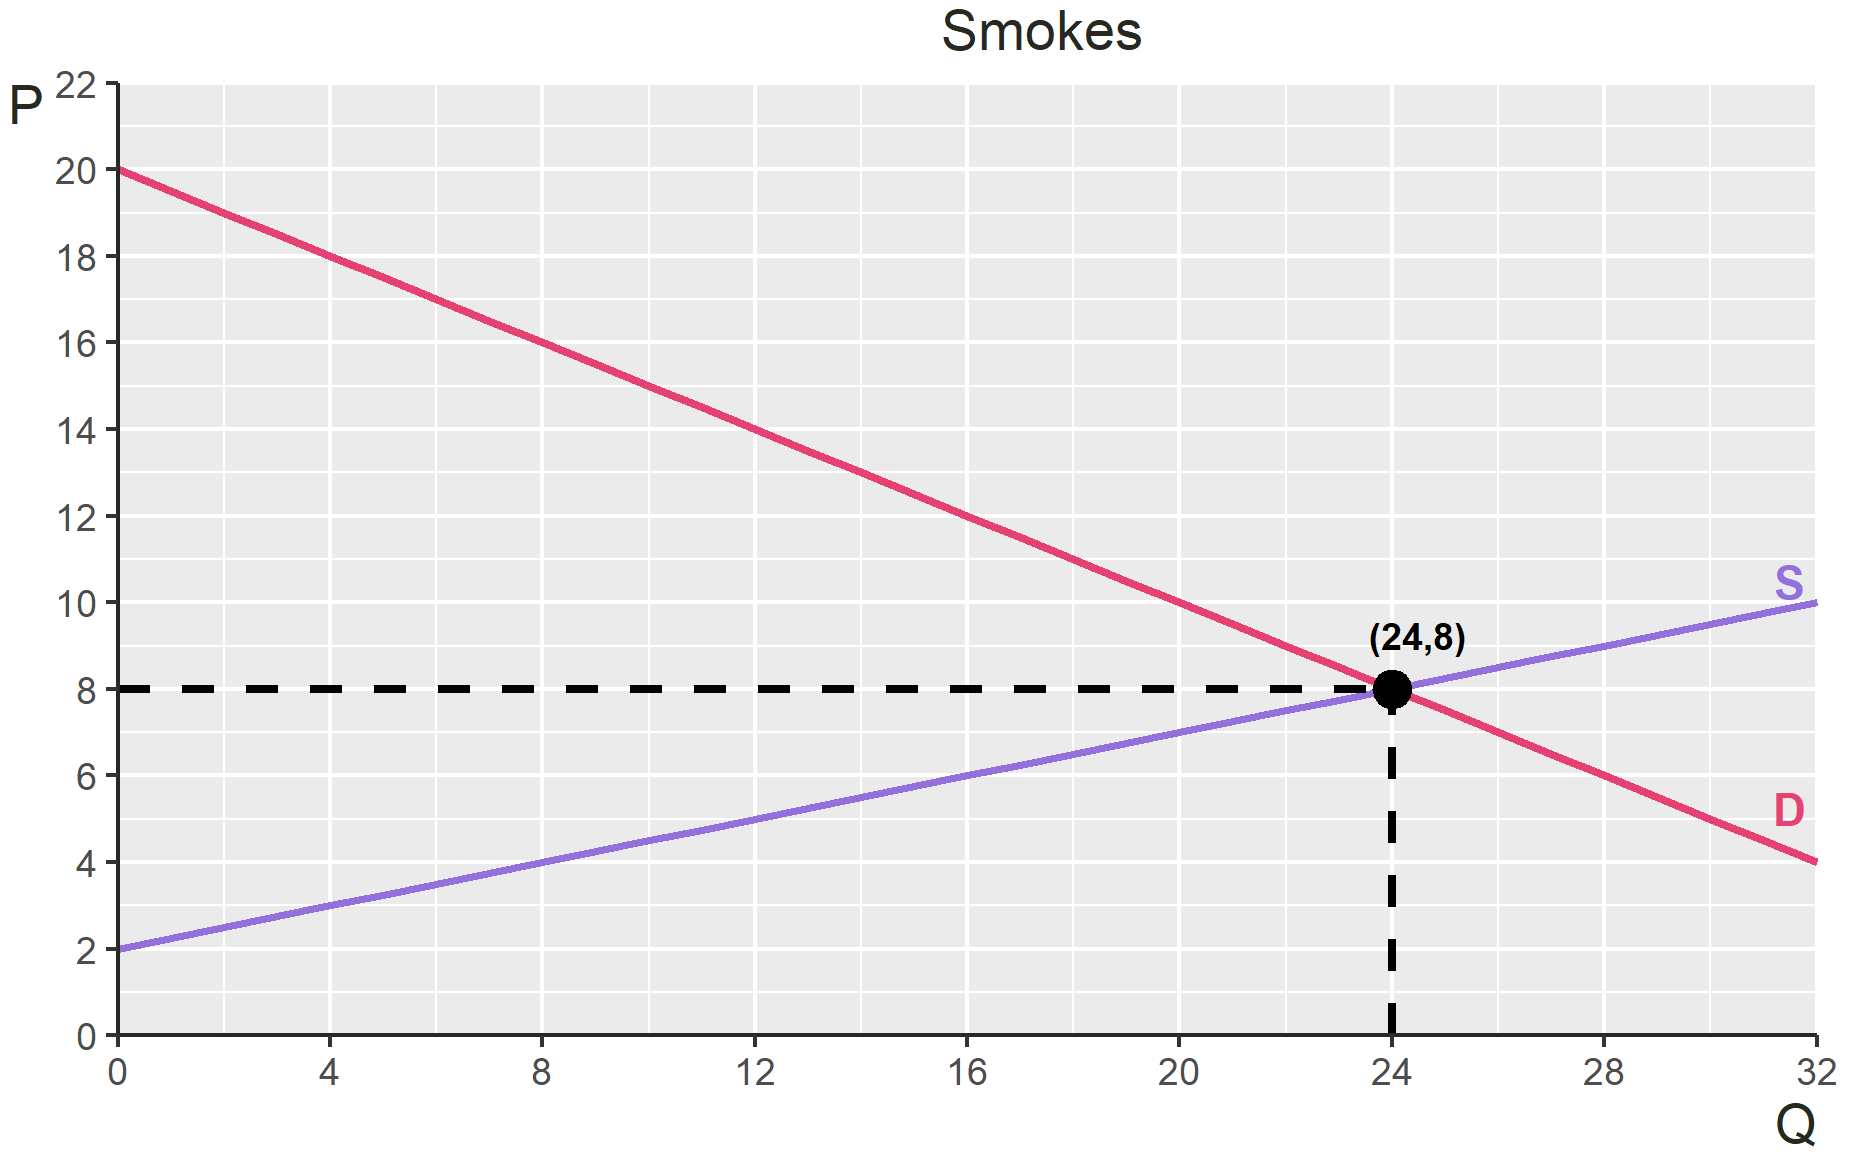
\includegraphics[width=7cm]{Dart mark.png}} & $[D]: \quad P=20-\frac{1}{2}Q$ \bigstrut \\
            & $[S]: \quad P=2+\frac{1}{4}Q$ \bigstrut\\
        \end{tabu}
        \end{table}
        \vspace{14mm}
        \item In order to discourage cigarette consumption, the government puts in a per-unit tax of \$6 in place. What happens in the market?
    \end{itemize}
\end{frame}

\begin{frame}{Example -- A Tax on Consumers}
    \begin{itemize}[<+->]
        \item With a per-unit tax of \$6, demand will shift down by 6: 
        \begin{table}
        \centering
        \renewcommand{\arraystretch}{3}
        \begin{tabu}{cc}
            \multirow{3}[3]{*}[1mm]{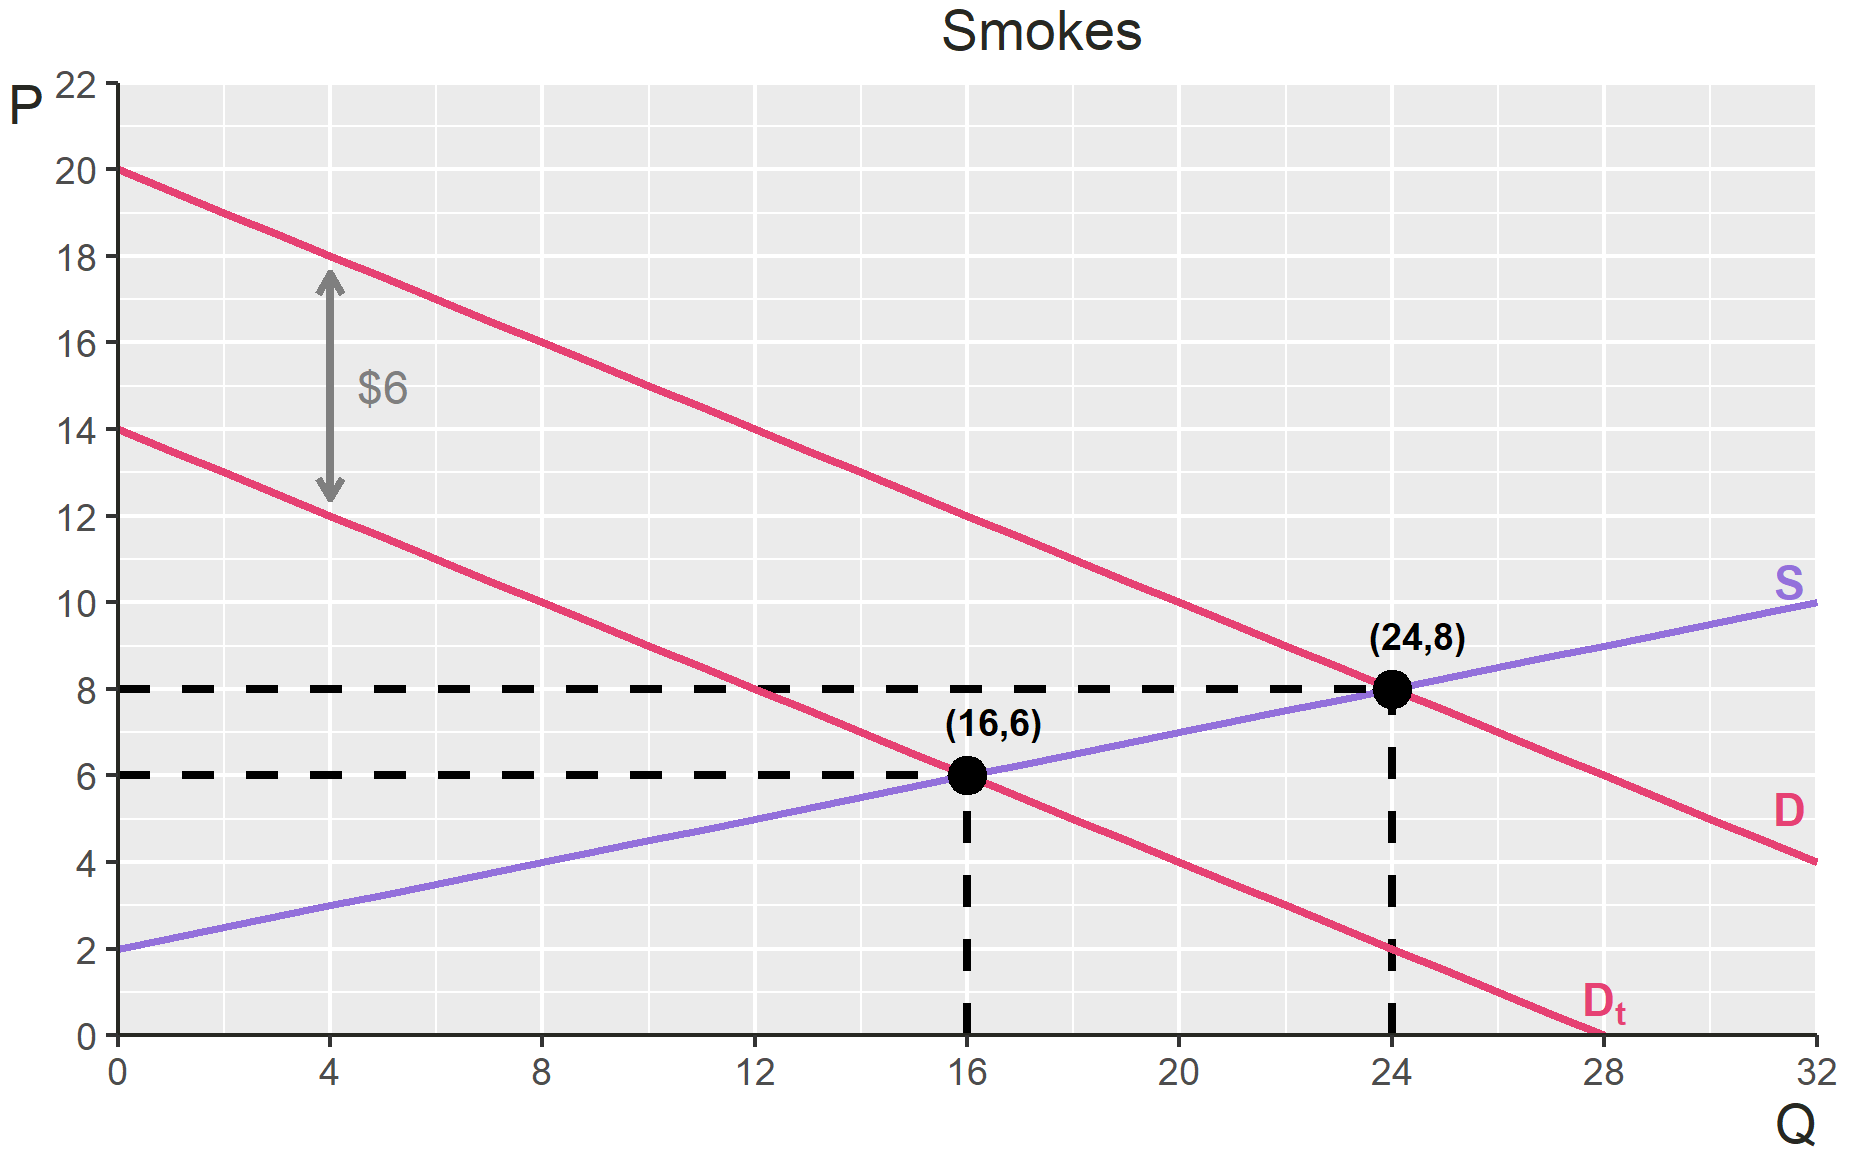
\includegraphics[width=7cm]{Dart tax.png}} & $[D]: \quad P=20-\frac{1}{2}Q$ \bigstrut \\
            & $[D_{t}]: \quad P=14-\frac{1}{2}Q$ \bigstrut \\
            & $[S]: \quad P=2+\frac{1}{4}Q$ \bigstrut\\
        \end{tabu}
        \end{table}
        \item Demand moves down from $D$ to $D_{t}$
    \end{itemize}
\end{frame}


\begin{frame}{Prices Paid Versus Prices Received}
    \begin{itemize}[<+->]
        \item In our regular equilibrium models, there is one price: the price paid by the consumers, which is the price received by producers
        \item With taxes and subsidies, this is no longer the case
        \begin{itemize}
            \item The government either took money from someone or gave money to someone
        \end{itemize}
        \item In the previous example, there was a $\$6$/unit tax, but the new ``equilibrium" price is $\$6$. Who is paying/receiving what?
        \item Suppose you go in to buy smokes...
        \begin{itemize}
            \item Story A: The cost is $\$12$, which you pay, and then the cashier has to give $\$6$ to the government, meaning they receive $\$6$
                \begin{itemize}
                    \item This is realistic, but makes it sound like the tax is on producers
                \end{itemize}
            \item Story B: The cost is $\$6$, which you pay the cashier. They keep all of it, and then on the way out, the tax man stops you and makes you pay $\$6$ for your pack of cigarettes
            \begin{itemize}
                \item Or you can think that you have to report this on your taxes
            \end{itemize}
            \item Note: Both these stories are equivalent/yield the same price paid/received
        \end{itemize}
    \end{itemize}
\end{frame}

\begin{frame}{Difference in Prices}
    \begin{figure}
        \centering
        \includegraphics[width=7cm]{Dart tax prices.png}
        \caption*{Correction: the graph is supposed to say ``price received by producers"}
    \vspace{-3mm}
    \end{figure}
    \begin{itemize}[<+->]
        \item In this example, the price paid by consumer is $\$12$, while the price received by the producer is $\$6$, leaving the $\$6$ tax going to the government
        \item Note: $(16, 6)$ is still worth calling the ``equilibrium" of the graph, the key difference is that there are now two prices worth talking about\footnote{$\$6$ could still be called the ``equilibrium price", but I will try to steer away from this terminology in this case}
    \end{itemize}
\end{frame}

\begin{frame}{Government Revenue\footnote{I use ``GR" rather than ``TR" for ``tax revenue", as to not get confused with ``total revenue"}}
    \begin{itemize}[<+->]
        \item Q: How much did the government collect in taxes? 
        \begin{itemize}
            \item A: They collected $\$6$/unit on 16 units, so 
            $$GR=16(6)=\$96$$
        \end{itemize}
        \visible<3->{
        \begin{figure}
            \centering
            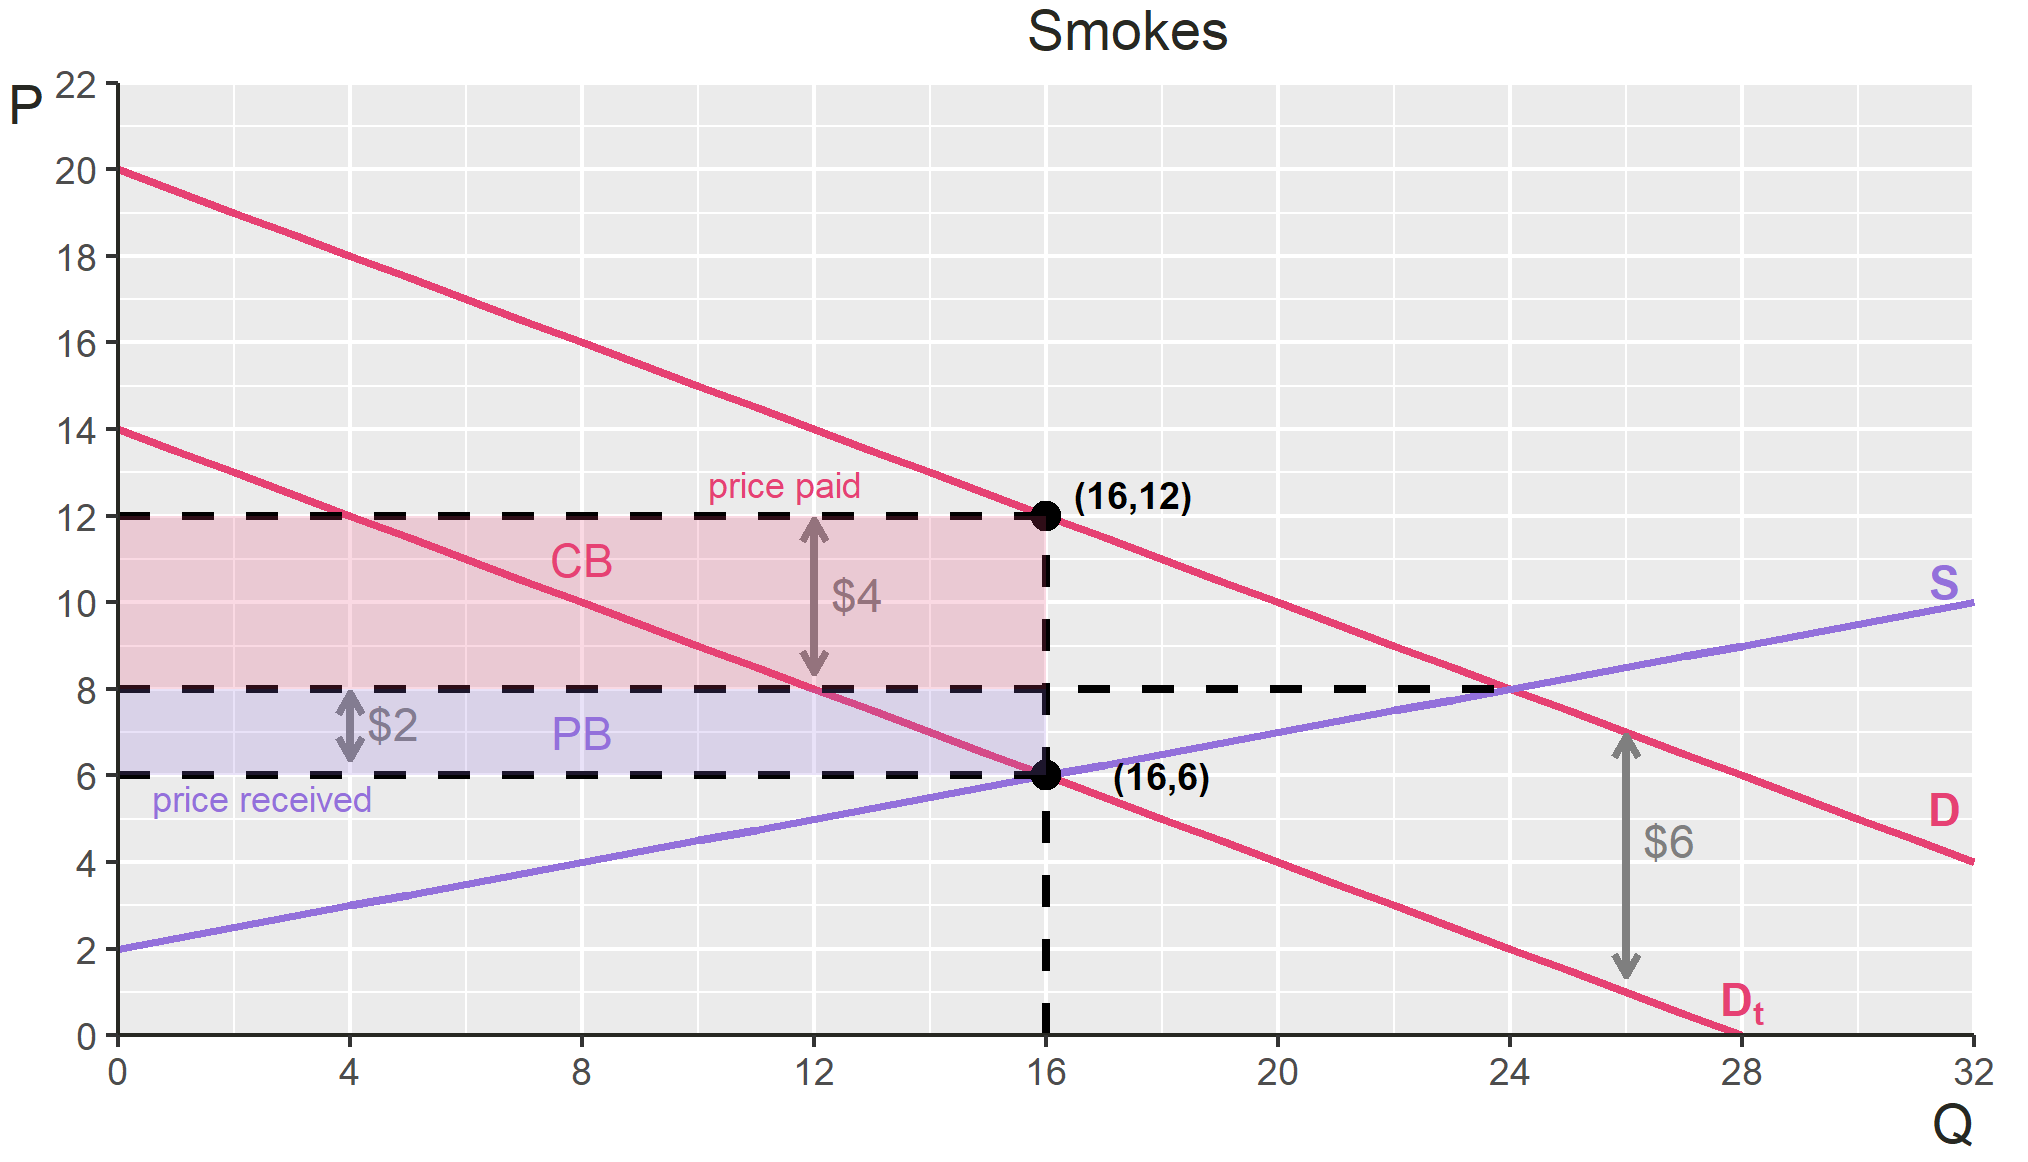
\includegraphics[width=6cm]{Dart tax gr.png}
        \end{figure}}
    \end{itemize}
\end{frame}


\begin{frame}{A Subsidy on Consumers}
    \begin{itemize}[<+->]
        \item How are subsidies different from taxes? 
        \item If we interpret a subsidy as a negative tax, then the $t$ from our previous derivation is negative
        \item Recall: if demand is given by $P=mQ+b$, then taxed demand is given by $P=mQ+b-t$
        \item So, if the subsidy, $s$, is equal to $-t$, then subsidized demand is given by $P=mQ+b+s$
        \begin{itemize}
            \item Subsidies just shift demand up!
        \end{itemize}
    \end{itemize}
\end{frame}

\begin{frame}{Example -- A Subsidy for Consumers}
    \begin{itemize}[<+->]
        \item If the government wanted to encourage consumption of solar panels, they could give a \$4000 per-unit subsidy on them, shown below:
        \begin{figure}
            \centering
            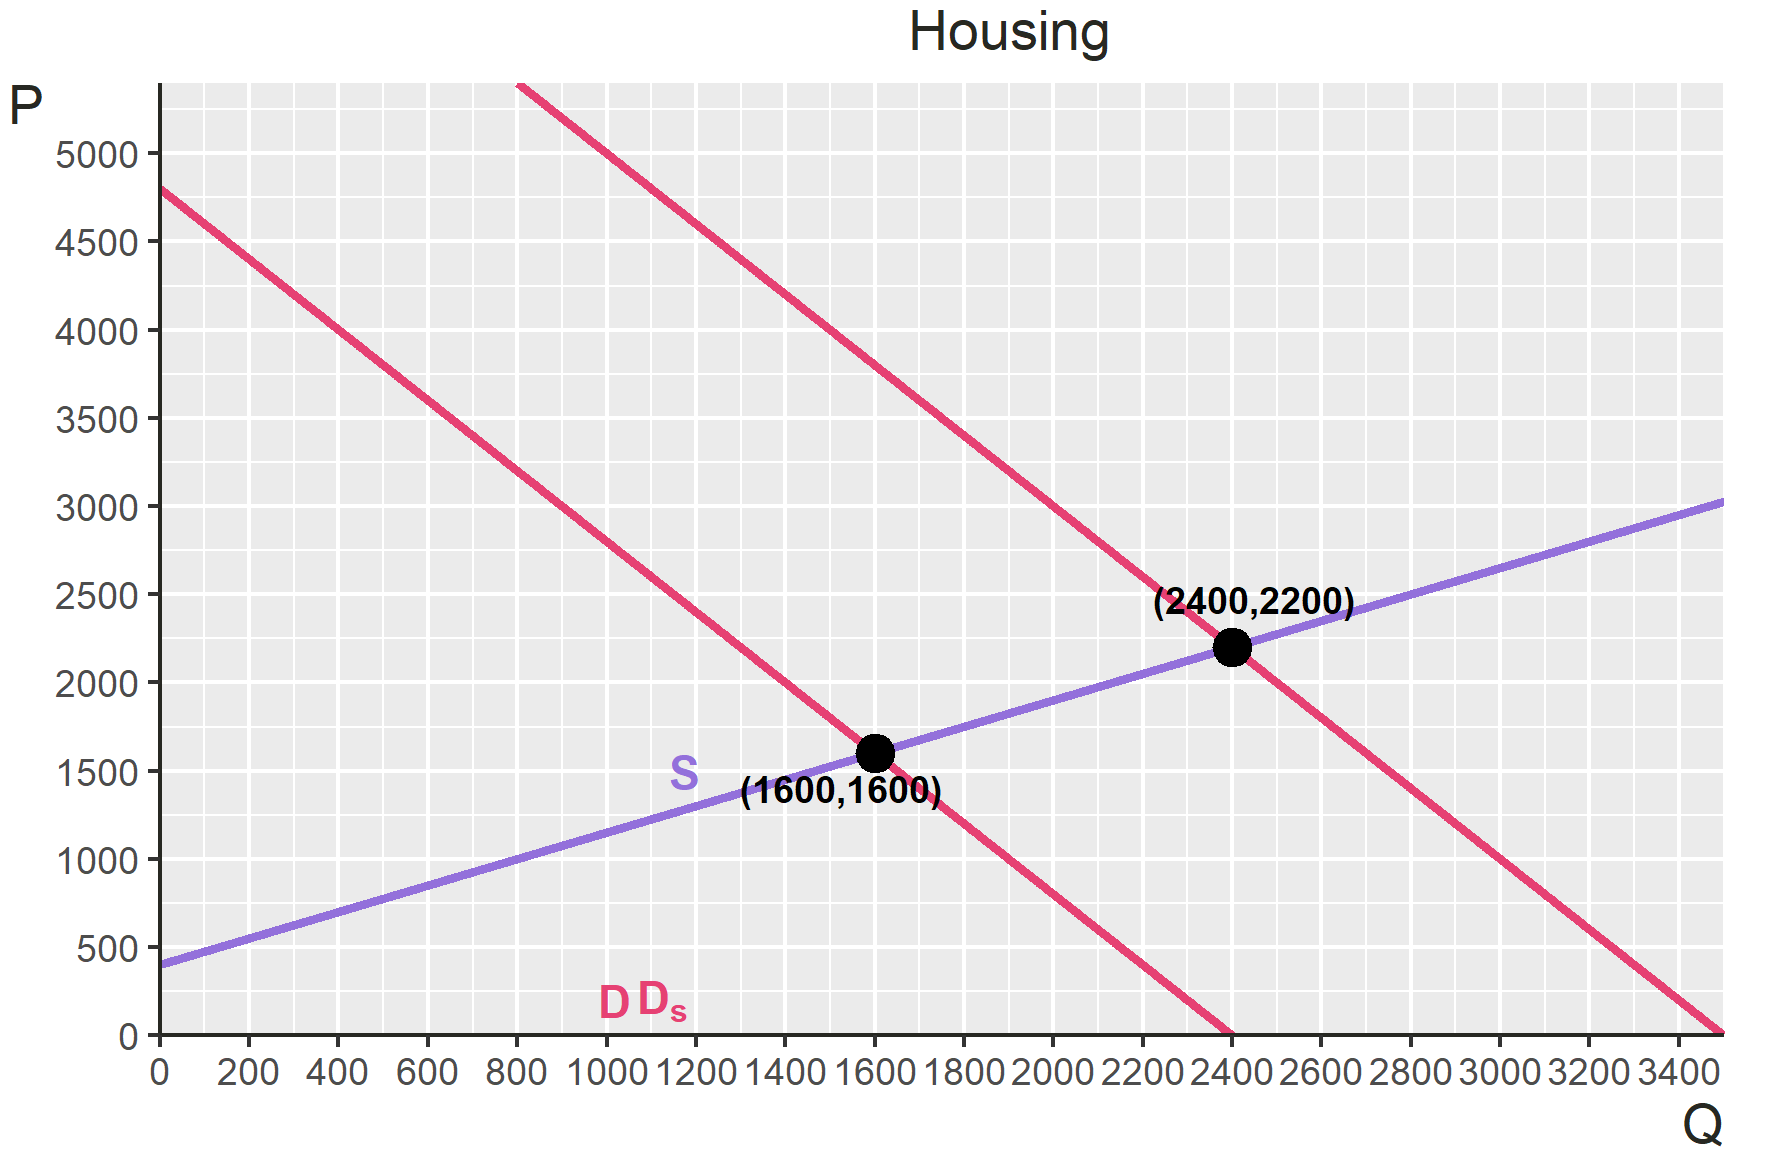
\includegraphics[width=8cm]{Solar sub.png}
            \caption*{The demand line shifts from $D$ to $D_{s}$ with the subsidy}
        \end{figure}
    \end{itemize}
\end{frame}

\begin{frame}{Difference in Prices -- Consumer Subsidy}
    \begin{itemize}[<+->]
        \item What is price paid/received?
        \begin{itemize}
            \item Story: you give the producer $\$8000$, and on the way out the tax man gives you $\$4000$, meaning you only spent $\$4000$ of your own money
        \end{itemize}
        \item Therefore, price paid by the consumer is $\$4000$, and price received by the producer is $\$8000$
        \begin{figure}
            \centering
            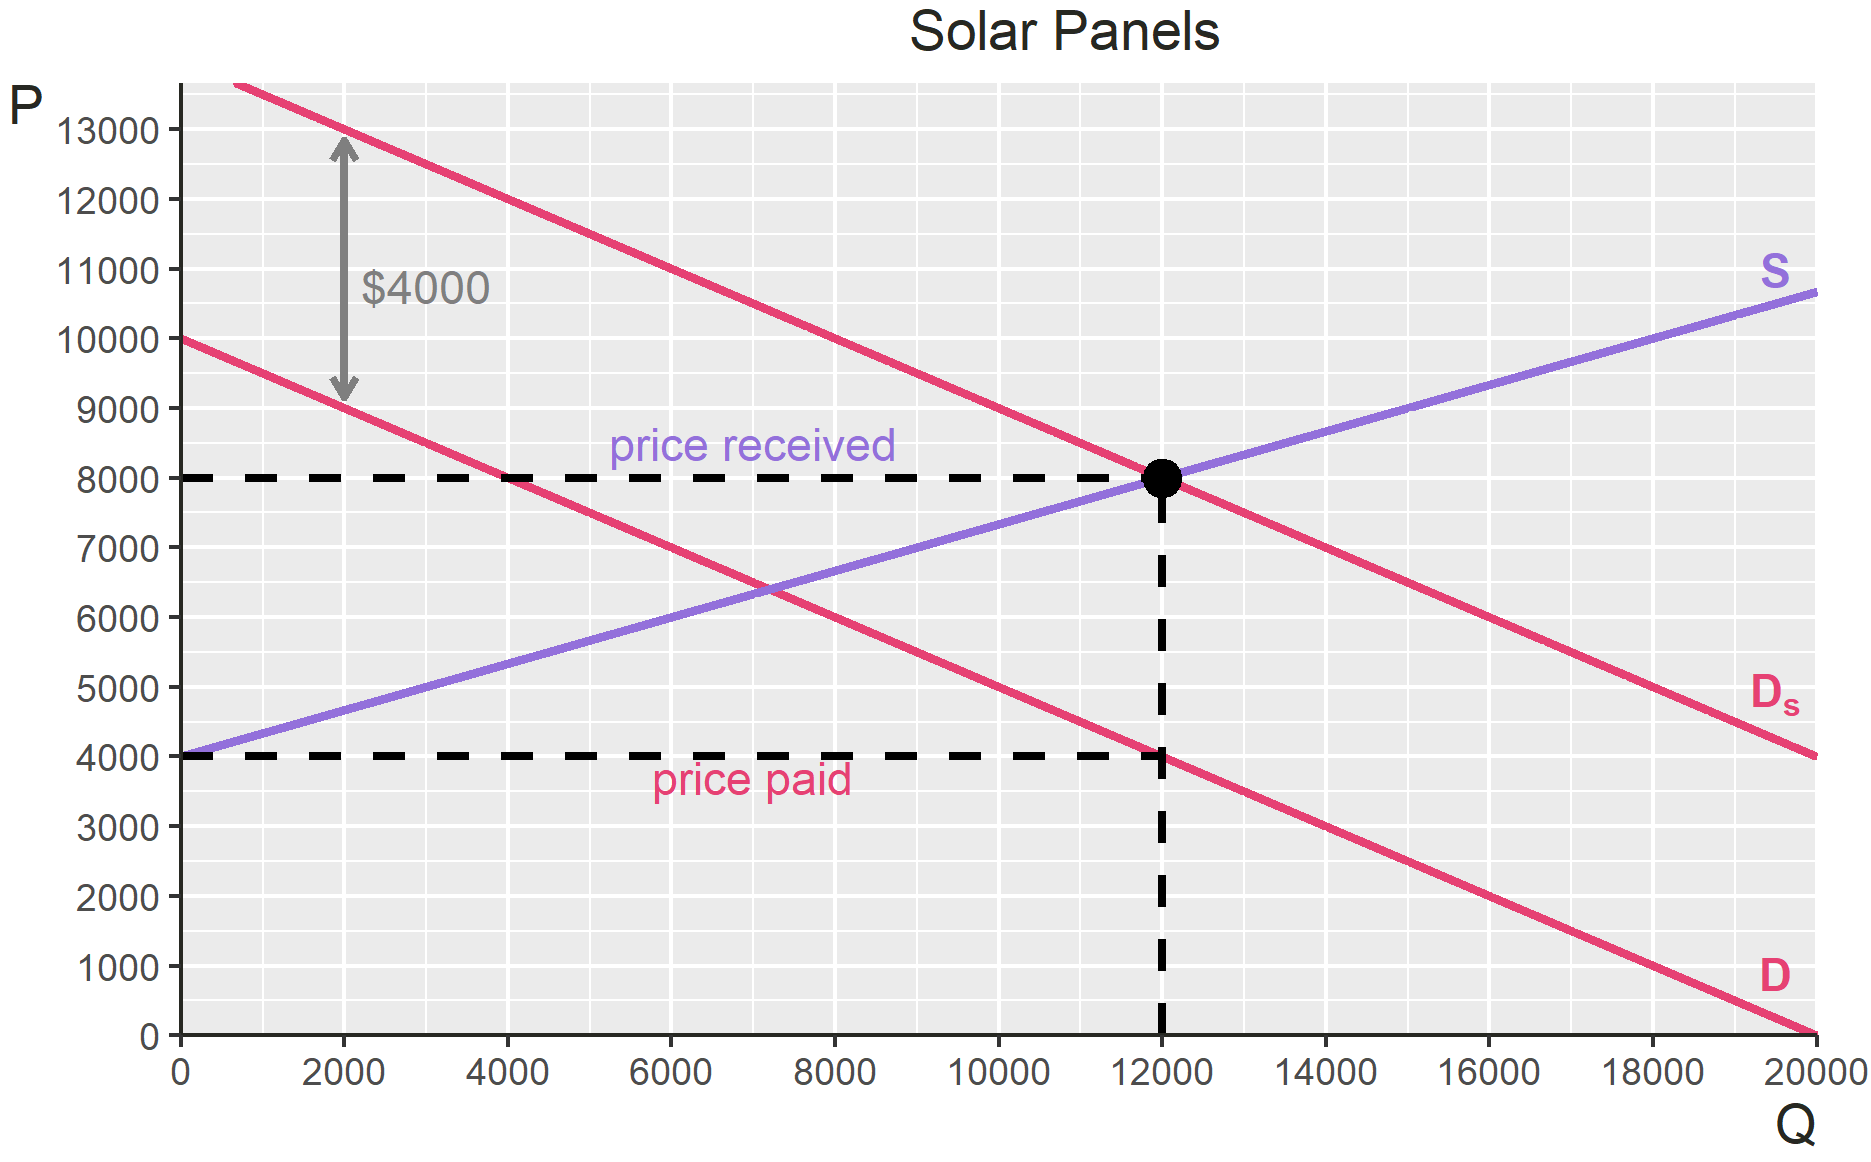
\includegraphics[width=8cm]{Solar sub prices.png}
        \end{figure}
    \end{itemize}
\end{frame}

\begin{frame}{Government Expenditure}
    \begin{itemize}[<+->]
        \item How much did the government spend?
        \begin{itemize}
            \item $\$4000$/unit subsidy times 12000 units traded, meaning $$GE=(4000)(12000)=\$48,000,000$$
        \end{itemize}
        \begin{figure}
            \centering
            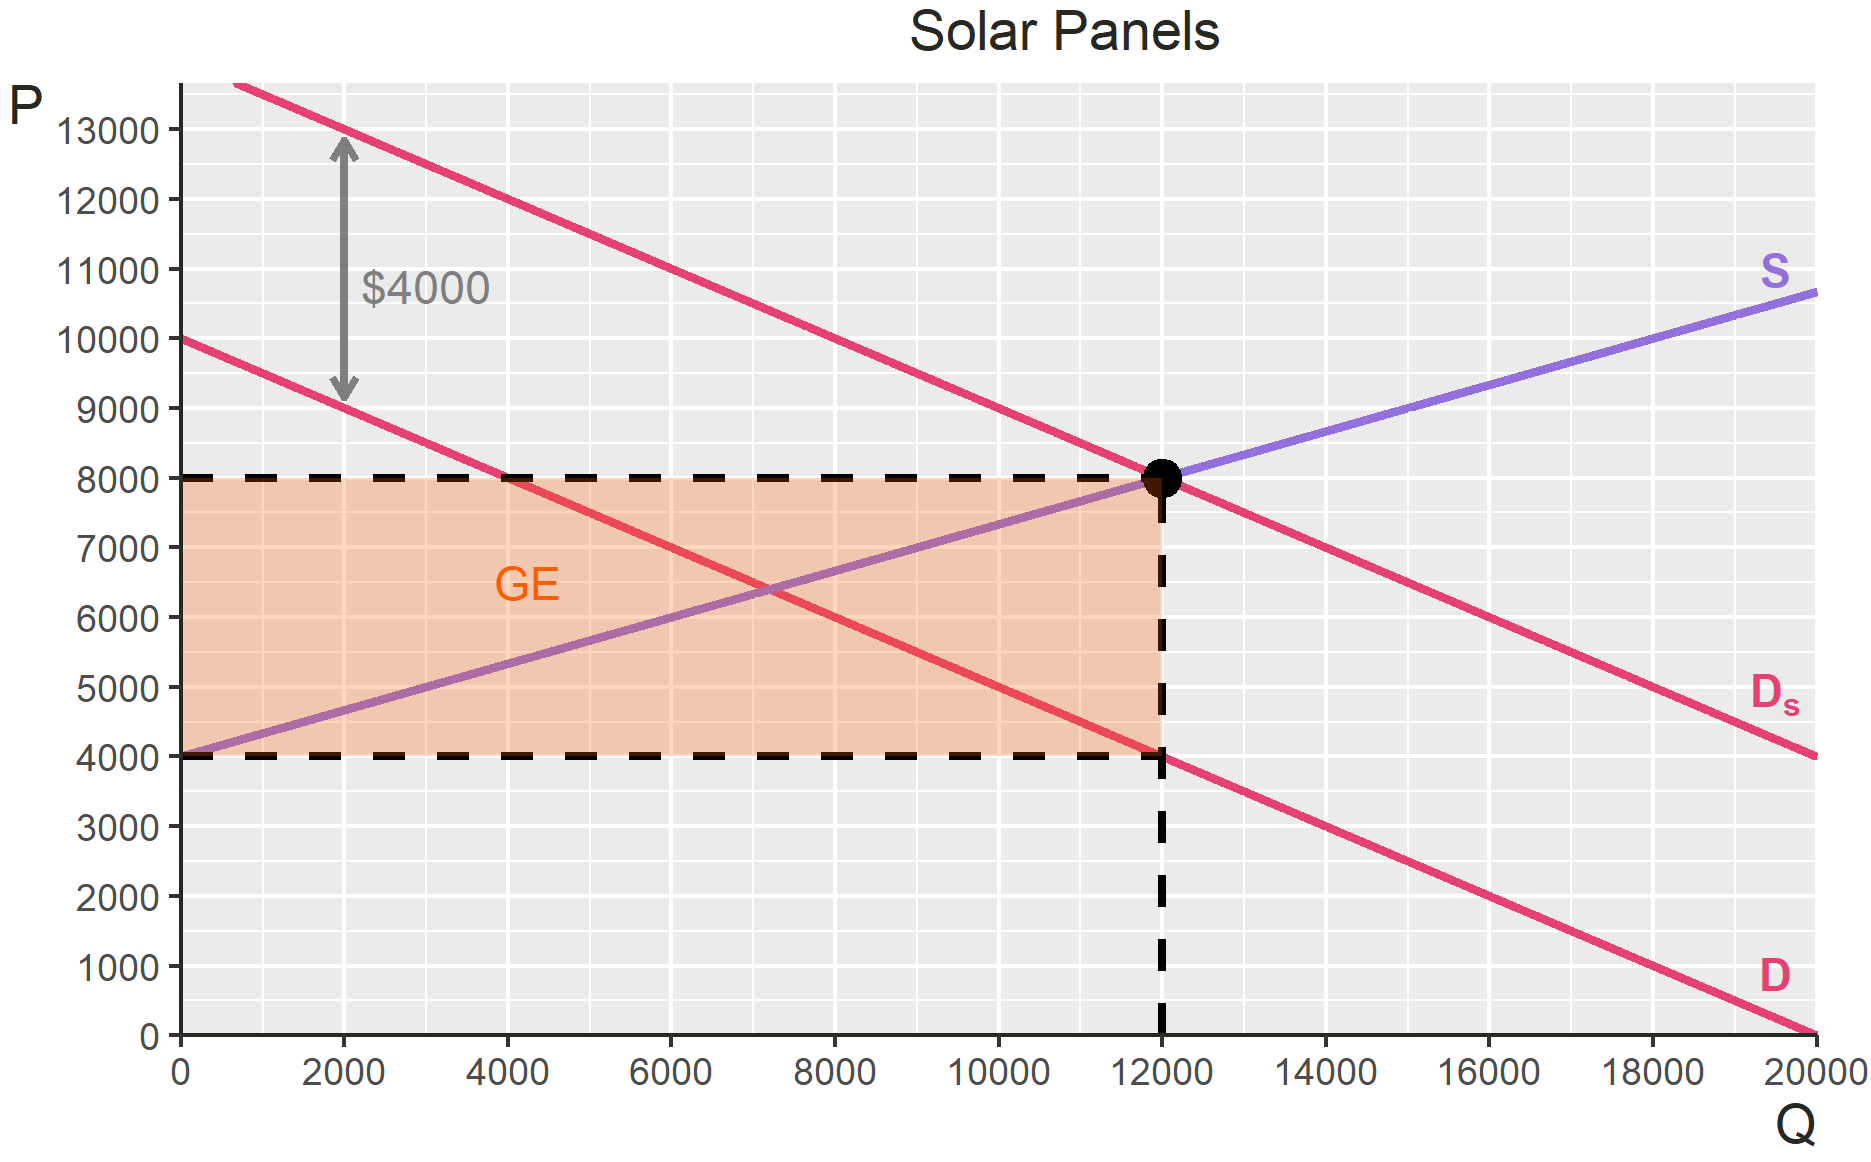
\includegraphics[width=7cm]{Solar sub ge.png}
        \end{figure}
    \end{itemize}
\end{frame}


\begin{frame}{Taxes and Subsidies on Production}
    \begin{itemize}[<+->]
        \item Why tax producers?
        \begin{itemize}
            \item We tax producers to discourage the \underline{production} of a good, rather than the consumption of said good
            \begin{itemize}
                \item Ex: smokestack pollutants, oil fracking, etc.
            \end{itemize}
            \item We subsidize producers to encourage production of a good
            \begin{itemize}
                \item Ex: wind turbines, agriculture (dairy, sugar), etc.
            \end{itemize}
        \end{itemize}
        \item Q: How do taxes and subsidies affect the supply curve?
        \item A: Taxes/subsides just shift supply down/up as well, but in a slightly different way
    \end{itemize}
\end{frame}

\begin{frame}{The Effect of a Tax on the Supply Curve}
    \begin{itemize}[<+->]
        \item Suppose supply for oil is given by 
        $$P=mQ+b\quad \iff \quad Q=\frac{P-b}{m}$$
        \item Adding a per-unit tax means that for each fixed value of Q, the price received by producers changes from $P$ to $P-t$
        $$Q=\frac{(P-t)-b}{m}$$
        \item Solving this for $P$ in terms of $Q$ yields
        $$P=mQ+b+t$$
        \item So what does the tax do?
        \begin{itemize}
            \item Shift supply up by $t$ units
        \end{itemize}
    \end{itemize}
\end{frame}

\begin{frame}{The Effect of a Subsidy on the Supply Curve}
    \begin{itemize}[<+->]
        \item Similarly, a subsidy for producers will shift supply \textit{down} by $t$ units
        \begin{itemize}
            \item This seems backwards, but remember that a ``negative supply shock", ``leftward shift in supply", or a ``decrease in supply" is actually akin to shifting supply upward, while shifting supply ``right" is akin to shifting it down
            \item This is just because supply is upward sloping
            \begin{itemize}
                \item Some graphs will help solidify this
            \end{itemize}
        \end{itemize}
        \item Thus, if supply is given by $P=mQ+b$, then subsidized supply is given by $P=mQ+b-s$, where $s$ is the positive subsidy
        \item It's still the case that taxes have a negative, regressive effect on supply/demand, while subsidies have a positive, stimulative effect on supply/demand
    \end{itemize}
\end{frame}

\begin{frame}{Example -- A Tax on Producers}
    \begin{itemize}[<+->]
        \item Suppose we want to discourage the rate at which businesses frack oil, and we do so by putting a \$40/unit tax on production
        \item This is visualized as
        \begin{figure}
            \centering
            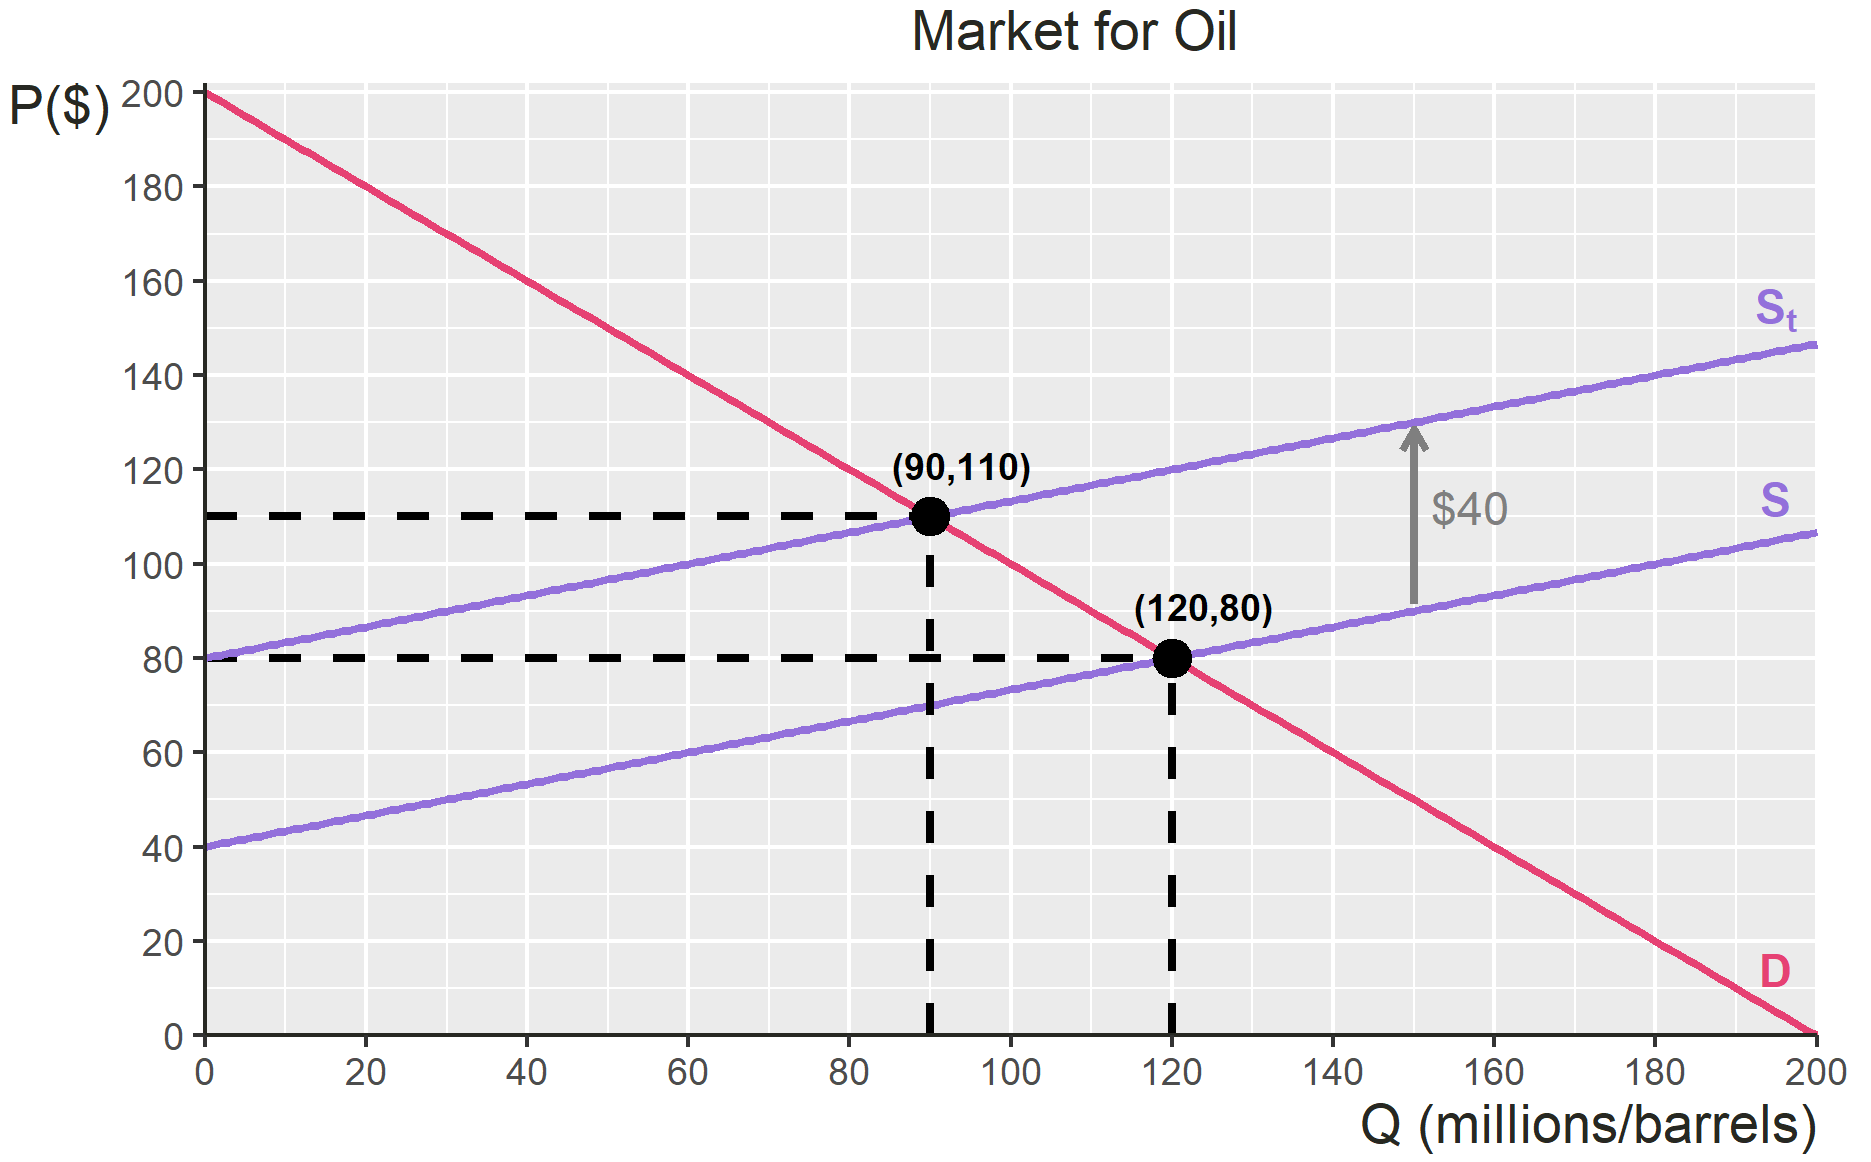
\includegraphics[width=8cm]{Oil tax.png}
            \caption*{The supply line shifts from $S$ to $S_{t}$ with the tax}
        \end{figure}
    \end{itemize}
\end{frame}

\begin{frame}{Example -- A Subsidy for Producers}
    \begin{itemize}[<+->]
        \item Suppose that, in order to encourage wind power prominence, the government provides a $\$600$/unit subsidy to producers
        \begin{figure}
            \centering
            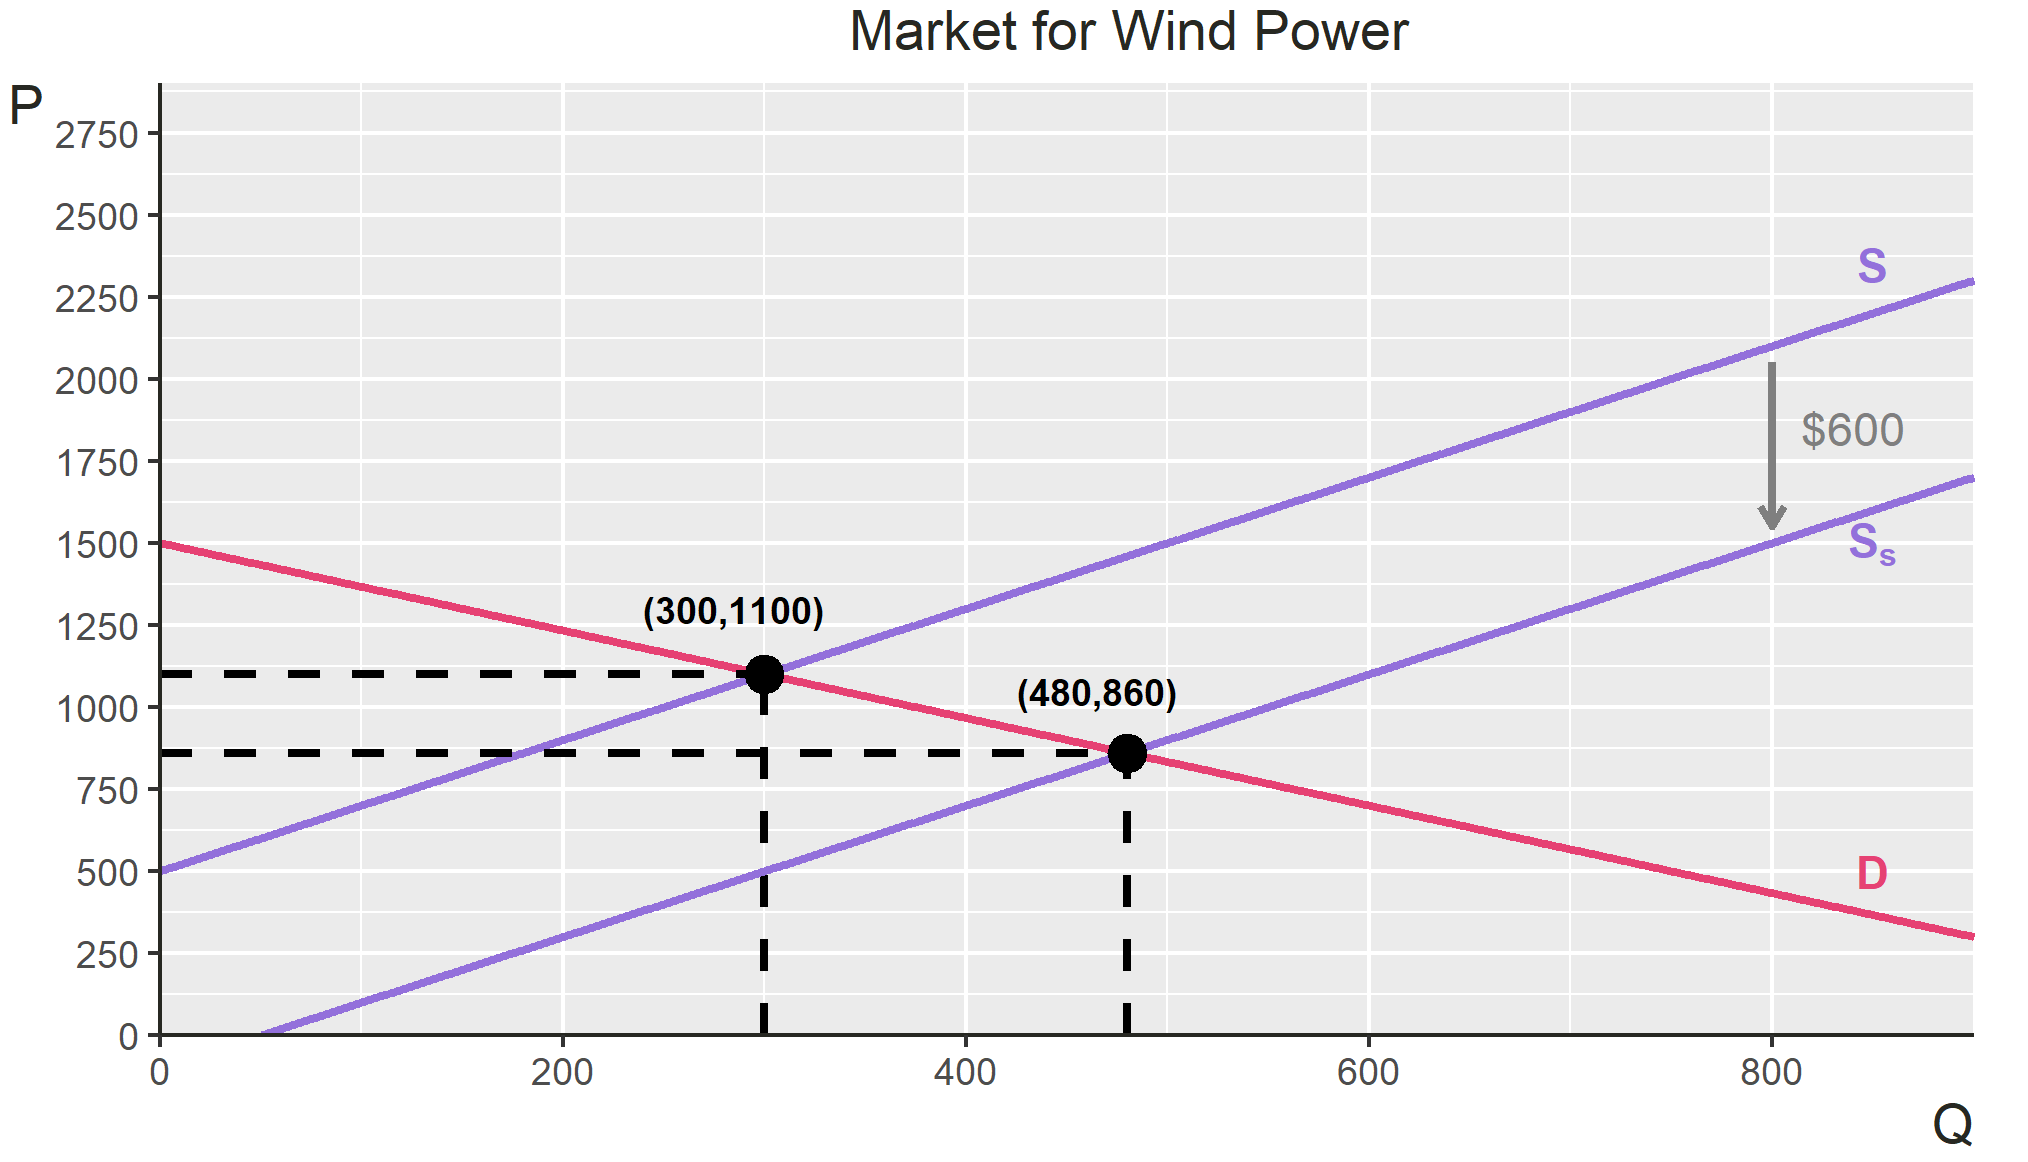
\includegraphics[width=8cm]{Wind sub.png}
            \caption*{The supply line shifts from $S$ to $S_{s}$ with the subsidy}
        \end{figure}
    \end{itemize}
\end{frame}

\begin{frame}{Food For Thought}
    \begin{itemize}[<+->]
        \item In the previous two graphs, what are price received and price paid?
        \item In the previous two graphs, what are government revenue and/or government expenditure?
        \item We will pick this up on Monday
        \item Questions?
    \end{itemize}
\end{frame}


\end{document}